\section{\filetotitle}\label{sec:sensitivity_analysis_in_photodynamics}
\textit{Commentary on: \fullcite{10.1021/acs.jctc.4c01008}}

The first published work of this thesis is focused on sensitivity analysis in photodynamics simulations from article \textit{Sensitivity Analysis in Photodynamics: How Does the Electronic Structure Control \textit{cis}-Stilbene Photodynamics?} in \textit{Journal of Chemical Theory and Computation}. A reaction video to this article by Pavlo O. Dral has been published on YouTube.\supercite{Z4qFv-QZMR8}

In computational photodynamics, nonadiabatic dynamics simulations are becoming standard tools to investigate the excited-state behavior of molecular systems. However, the accuracy of these simulations strongly depends on the underlying electronic structure method used to compute the potential energy surfaces and nonadiabatic couplings. Researchers often face the challenge of selecting an appropriate electronic structure method, as different methods can yield varying results for the same system.\supercite{10.1021/acs.jctc.3c00908,10.1021/acs.jctc.2c00968,10.1021/acs.jctc.9b00282} This work exposes this challenge by performing a sensitivity analysis on the photodynamics of \textit{cis}-stilbene, a prototypical photoisomerization system. \textit{cis}-stilbene undergoes photoinduced isomerization around its central double bond, leading to the formation of either the trans isomer (\textit{trans}-stilbene) or a cyclized product called \acrfull{dhp}, making it an ideal candidate for studying nonadiabatic dynamics and the influence of electronic structure methods. The three isomers are depicted in Fig~\ref{fig:stilbene_isomers}.
\begin{figure}[H]
\centering
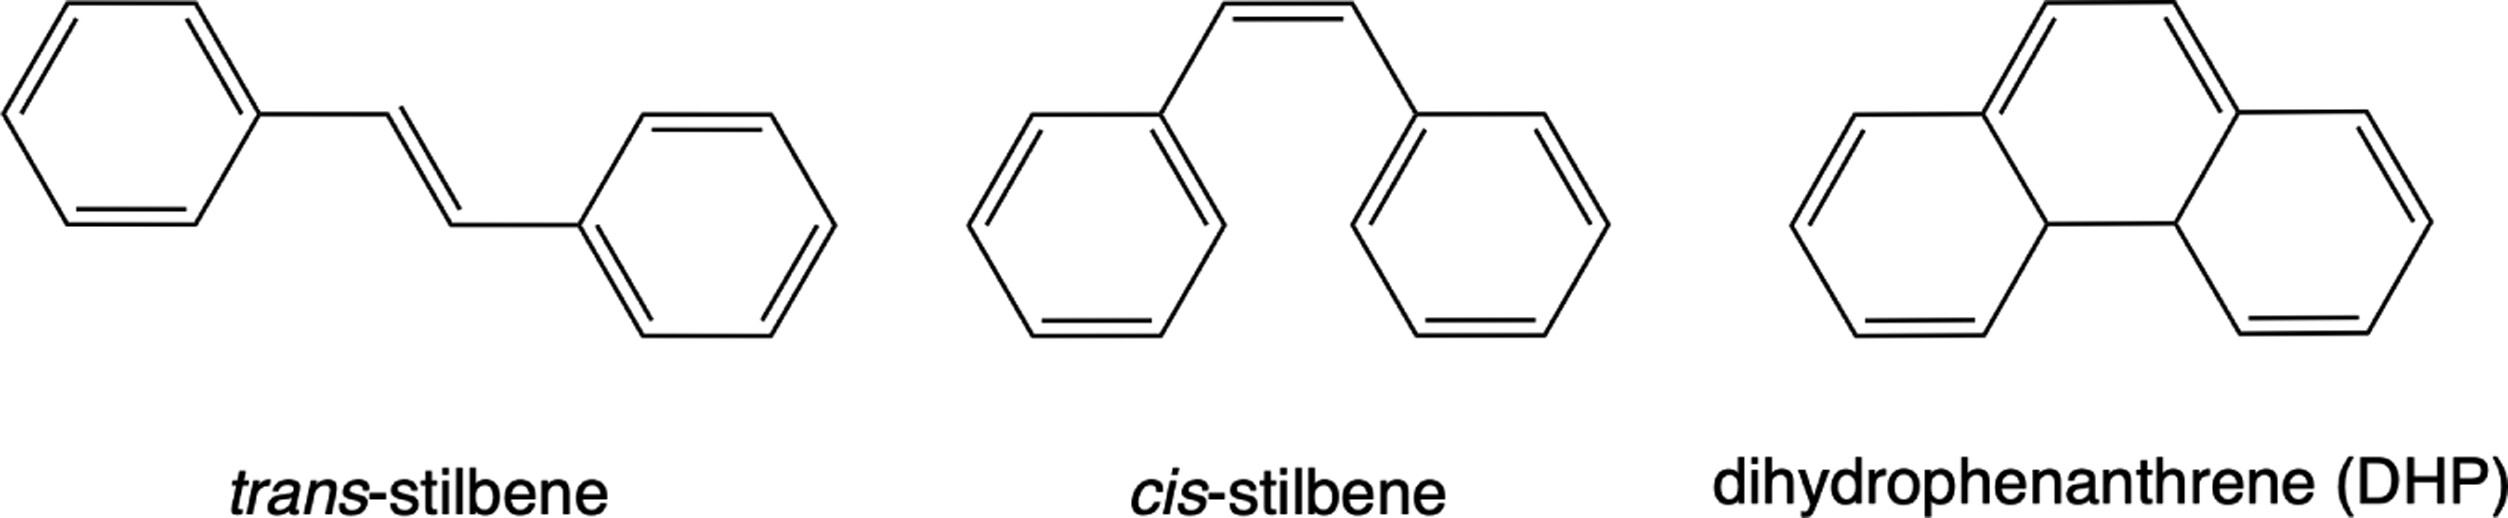
\includegraphics[width=0.9\linewidth]{chapters/05-Primary_Scientific_Contributions/sections/images/images_large_ct4c01008_0001}
\caption{The three stilbene isomers.}
\label{fig:stilbene_isomers}
\end{figure}
The study uses the \acrfull{fssh} method, described in Sec~\ref{sec:fewest_switches}, to simulate the nonadiabatic dynamics of \textit{cis}-stilbene using various electronic structure methods. For the low-level method, semiempirical OM3-MRCISD is employed, while for the high-level methods, \acrfull{sa-casscf} and \acrfull{sa-caspt2} were are used. Using these methods, the study calculates the excited-state lifetimes and populations, quantum yields for photoisomerization and cyclization, and \acrfull{trpes}. The results are then compared with the experimental data to assess the accuracy of each electronic structure method.

To start the sensitivity analysis, the study first establishes the investigated \acrshort{pes} and all the important features that influence the photodynamics of \textit{cis}-stilbene. Upon excitation to the first excited state (S$_1$) there are two main relaxation pathways. The first pathway leads to through the \textit{cis}-stilbene S$_1$ minimum to an energetically close conical intersection between S$_1$ and the ground state (S$_0$) that facilitates the isomerization to \acrshort{dhp} or back to \textit{cis}-stilbene. The second pathway leads through another S$_1$ minimum to four conical intersections between S$_1$ and S$_0$ that facilitate the isomerization to \textit{trans}-stilbene or back to \textit{cis}-stilbene. Note that all of the conical intersections are energetically accessible from the S$_1$ Franck--Condon region. The \acrshort{pes} features on all three electronic structure levels are qualitatively similar, with no seemingly preferred pathway. The schematic representation of the \acrshort{pes} features is shown in Fig~\ref{fig:pes_features_stilbene}.
\begin{figure}[H]
\centering
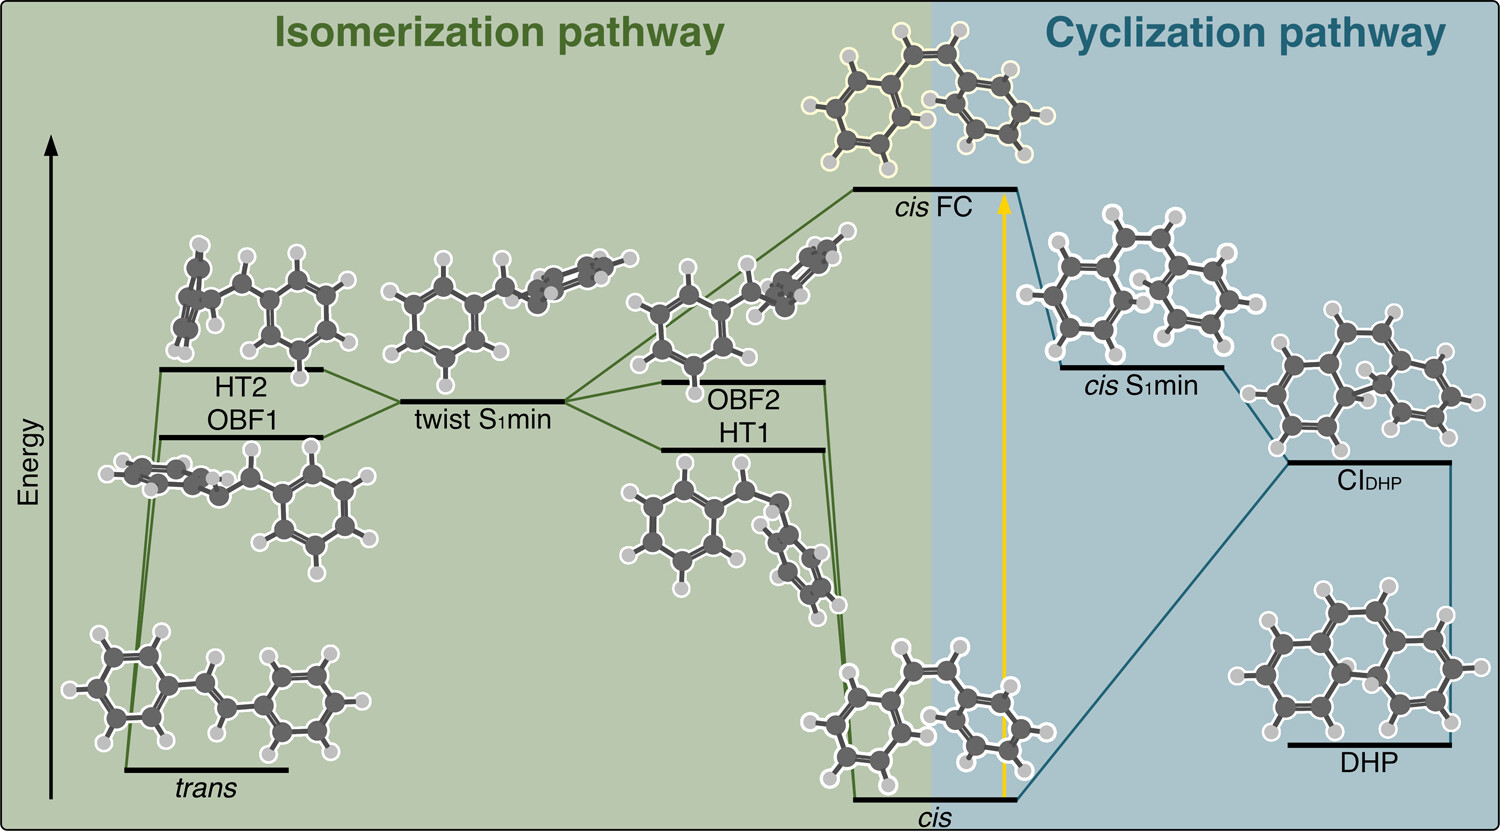
\includegraphics[width=\linewidth]{chapters/05-Primary_Scientific_Contributions/sections/images/images_large_ct4c01008_0003}
\caption{Schematic representation of the potential energy surface features of \textit{cis}-stilbene relevant to its photodynamics. The diagram illustrates the two main relaxation pathways from the S$_1$ excited state: one leading to the formation of \acrshort{dhp} via a conical intersection (CI) accessible from the S$_1$ minimum, and the other leading to \textit{trans}-stilbene via multiple conical intersections.}
\label{fig:pes_features_stilbene}
\end{figure}
After characterizing the stationary points, nonadiabatic dynamics simulations were performed using different electronic structure methods. Quantum yields and excited-state lifetimes obtained from these simulations are summarized in Tab~\ref{tab:sensitivity_analysis_results}.
\begin{table}[H]
    \centering
    \caption{Summary of the photodynamics results for \textit{cis}-stilbene using different electronic structure methods. The quantum yields for \textit{cis}-stilbene ($\phi_{\symit{cis}}$), \textit{trans}-stilbene ($\phi_{\symit{trans}}$), and \acrshort{dhp} ($\phi_{\symrm{DHP}}$) formation, along with the excited-state lifetime ($\tau$), are presented. The results from previous studies and experimental data are also included for comparison.}
    \label{tab:sensitivity_analysis_results}
    \begin{tabular}{lcccc}
        \hline
        Level of Theory&$\phi_{\symit{cis}}$&$\phi_{\symit{trans}}$&$\phi_{\symrm{DHP}}$&$\tau$ (fs)\\
        \hline
        OM3-MRCISD(12,17) (LZSH)& $0.48\pm0.05$&$0.52\pm0.05$&$0.00\pm0.00$ &$321\pm10$\\
        SA2-CASSCF/SVP&$0.29\pm0.06$&$0.68\pm0.06$&$0.03\pm0.02$&$360\pm6$\\
        XMS-SA3-CASPT2/cc-pVDZ&$0.55\pm0.14$&$0.02\pm0.04$&$0.43\pm0.14$&$295\pm10$\\
        XMS-SA2-CASPT2/cc-pVDZ&$0.91\pm0.07$&$0.00\pm0.00$&$0.09\pm0.07$&--\\
        \hline
        XMS-SA3-CASPT2(2,2)/cc-pVDZ\supercite{10.1021/jacs.2c12266}&$0.55\pm0.14$&$0.04\pm0.10$&$0.41\pm0.14$& $572\pm16$\\
        OM3-MRCISD(12,17)\supercite{10.1038/s41557-022-01012-0}&0.48&0.52&0.0&$\approx500$\\
        SA2-CASSCF(2,2)/6-31G*\supercite{10.1021/acs.jpcb.0c03344}&$0.45\pm0.04$&$0.52\pm0.04$&$0.04\pm0.01$&$520\pm40$\\
        \hline
        Experiment in Solvents\supercite{10.1021/ja00076a041,10.1021/acs.jpca.8b04011}&0.47-0.59&0.35-0.39&0.05-0.08&380-1650\\
        \hline
    \end{tabular}
\end{table}
The results show significant differences in the quantum yields and excited-state lifetimes depending on the electronic structure method used. The OM3-MRCISD method predicts a nearly equal distribution between \textit{trans}-stilbene and \textit{cis}-stilbene formation, with no \acrshort{dhp} formation. Whereas the SA2-CASSCF method predicts a higher quantum yield for \textit{trans}-stilbene formation, with a small amount of \acrshort{dhp} formation. And finally, the XMS-SA3-CASPT2 method predicts a high quantum yield for \acrshort{dhp} formation, with a low quantum yield for \textit{trans}-stilbene formation. The XMS-SA2-CASPT2 method turns out to be inadequate for describing the photodynamics of \textit{cis}-stilbene, as it predicts almost none population transfer to the ground state. The excited-state lifetimes also vary, but all methods predict lifetimes comparable to the lower end of the experimental range. The quantum yields in the table above lead to a conclusion that the choice of electronic structure method has a profound impact on the predicted photodynamics. The simple static picture of the \acrshort{pes} features does not provide enough information to predict the outcome of the dynamics simulations, as all methods show similar \acrshort{pes} features but yield different photodynamics results.

The study also analyzes the \acrshort{trpes} obtained from the simulations (Fig~\ref{fig:stilbene_spectra}) and compares them with experimental data. The \acrshort{trpes} provide insights into the electronic structure and dynamics of the system, and the results show that different electronic structure methods yield spectra that, except for XMS-SA2-CASPT2, exhibit features consistent with experimental observations. This observation further emphasizes the importance of selecting an appropriate electronic structure method, since the \acrshort{trpes} alone cannot be used to determine which method provides the most accurate description of the photodynamics.
\begin{figure}[H]
\centering
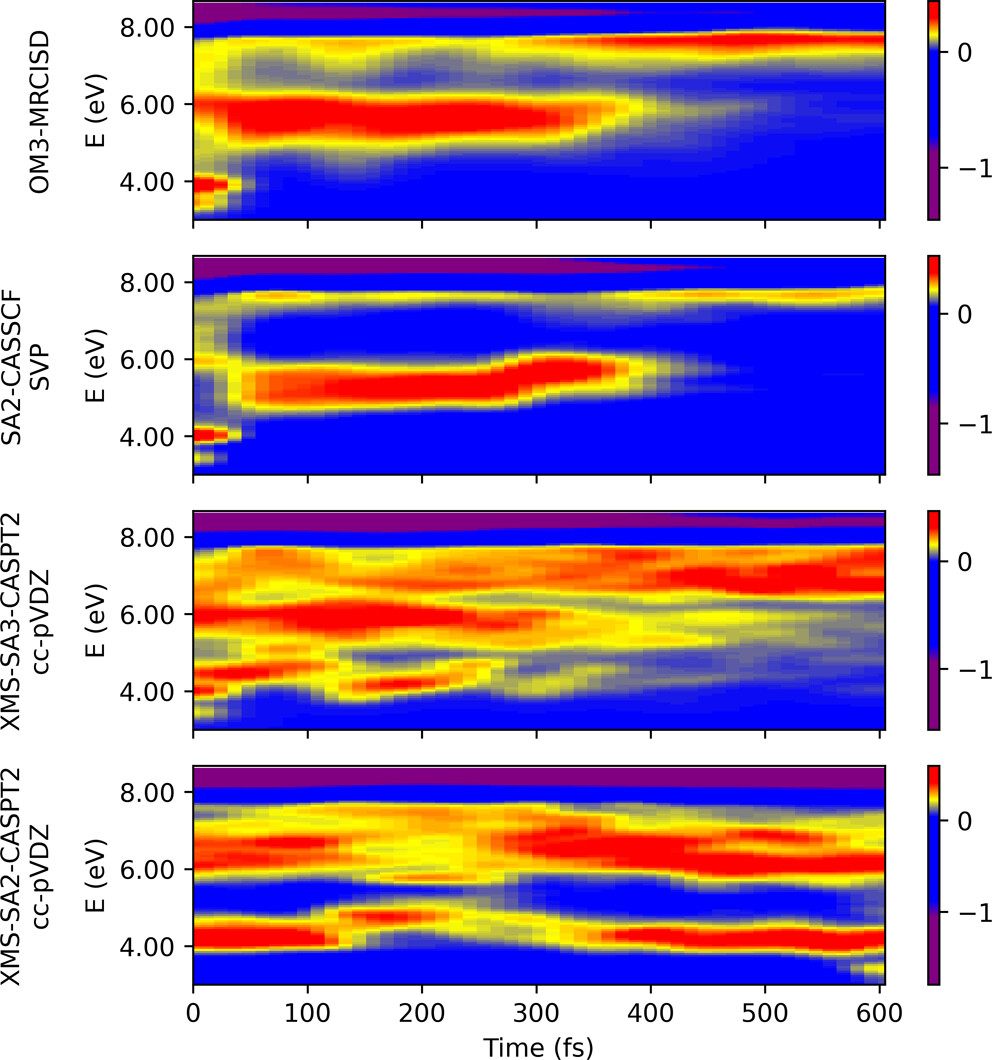
\includegraphics[width=0.7\linewidth]{chapters/05-Primary_Scientific_Contributions/sections/images/images_large_ct4c01008_0009}
\caption{Simulated \acrshort{trpes} for surface hopping dynamics with various electronic structure methods}
\label{fig:stilbene_spectra}
\end{figure}
Now the results beg a question: How to choose the right electronic structure method for nonadiabatic dynamics simulations? The study suggests that a combination of factors should be considered when selecting an electronic structure method. Of course, running several dynamics simulations with different methods and comparing the results with experimental data is the most straightforward approach. However, this can be computationally expensive and time-consuming. Therefore, the study recommends using a cheap method, like OM3-MRCISD, and artificially perturbing it using a bias potential to mimic the behavior of higher-level methods. This approach allows for a more efficient exploration of the sensitivity of the photodynamics to changes in the electronic structure, providing insights into the reliability of the chosen method. This approach was applied to the \textit{cis}-stilbene system, and the results showed that small perturbations to the OM3-MRCISD \acrshort{pes} could lead to significant changes in the predicted quantum yields and excited-state lifetimes, confirming the sensitivity of the system to the electronic structure method.

Overall, this work highlights the importance of sensitivity analysis in photodynamics simulations and provides valuable insights into the influence of electronic structure methods on the predicted photodynamics of \textit{cis}-stilbene. The findings and suggestions presented in this study can guide researchers in selecting appropriate electronic structure methods for nonadiabatic dynamics simulations, ultimately leading to more accurate and reliable predictions of excited-state behavior in molecular systems.
